\documentclass[compress]{beamer}
\batchmode

\usepackage{tikz}
\usetikzlibrary{shapes,snakes,arrows,scopes,positioning,calc}
%\usetikzlibrary{positioning}
%\usetikzlibrary{shapes,arrows,scopes}
\usepackage{amsmath,amssymb,bbm,epsfig,calc,color,ifthen,capt-of}
\usepackage[round]{natbib}
\usepackage{enumitem}
%\usepackage{harvard}
%\citationmode{abbr}
%\citationstyle{dcu}


\let\oldcite=\cite                                                              
\renewcommand{\cite}[1]{\textcolor{violet}{\textit{(\oldcite{#1})}}}


%\usepackage[absolute,overlay]{textpos}

% Configuration

%\usetheme{Madrid}
%\usetheme{Warsaw}
\useoutertheme{shadow}
\useinnertheme[shadow=true]{rounded}
\usecolortheme{rose}
\setbeamertemplate{blocks}[rounded][shadow=false]
\beamertemplatenavigationsymbolsempty
\setbeamersize{text margin left=5mm,text margin right=5mm} 

\definecolor{headfq}{RGB}{255,0,0}   %red
\definecolor{headbg}{RGB}{249,196,95}  
%\definecolor{titlebg}{RGB}{0,153,79} %green
\definecolor{titlebg}{RGB}{49,91,125} %steel blue
%\definecolor{backse}{RGB}{0,102,52} %green
\definecolor{backse}{RGB}{70,130,180} %steel blue
\definecolor{Periwinkle}{RGB}{153,146,172}

\definecolor{screenfoot}{RGB}{224,224,224}
\definecolor{letterfoot}{RGB}{153,0,76}


\setbeamercolor{Periwinkle}{fg=Periwinkle,bg=Periwinkle!50!white}
\setbeamercolor{equation}{fg=example text.fg,bg=example text.fg!20!bg}
\setbeamercolor{frametitle}{fg=white,bg=titlebg}
\setbeamercolor{title}{fg=white,bg=titlebg}
\setbeamercolor{palette}{bg=titlebg}
\setbeamercolor{section in head/foot}{fg=white,bg=titlebg}
\setbeamercolor{footcolor}{fg=white,bg=titlebg}

\setbeamertemplate{section in head/foot}{\colorbox{backse}{\insertsectionhead}}
\setbeamertemplate{section in head/foot shaded}{\color{fg!50!bg}\insertsectionhead}
\setbeamerfont*{title}{series=\bfseries}

\newcommand*\circled[1]{\tikz[baseline=(char.base)]{
 			\node[shape=circle,draw=green,fill=green,minimum size=6mm] (char) {#1};}}
            
\newcommand*\triangled[1]{\tikz[baseline=(char.base)]{
 			\node[shape=regular polygon,regular polygon sides=3,draw=red,fill=red,inner sep=1pt] (char) {#1};}}            


\setbeamertemplate{headline}{%
\leavevmode%
  \hbox{%
    \begin{beamercolorbox}[wd=\paperwidth,ht=2.8ex,dp=0.525ex]{palette}%
    \hspace*{1em}
    \insertsectionnavigationhorizontal{\paperwidth}{}{\hskip0pt plus1filll}
     \end{beamercolorbox}%
  }
}


\setbeamertemplate{frametitle}
{
\vskip-1pt
  \leavevmode
  \hbox{%
  \begin{beamercolorbox}[wd=\paperwidth,ht=2.5ex,dp=0.5ex]{frametitle}%
    %\includegraphics[height=0.35in]{logL2E.png}\hfill
    \raggedleft
    \textbf{\LARGE\insertframetitle} \hspace*{0.5em}
  \end{beamercolorbox}
  }%
}


\setbeamertemplate{footline}{%
   \leavevmode%
%\rule{2cm}{0.2cm}‎
  \hbox{%
  \begin{beamercolorbox}[wd=\paperwidth,ht=2.5ex,dp=1.0ex]{footcolor}%
    \raggedleft
    \insertpagenumber  \hspace*{0.5em}
  \end{beamercolorbox}%
  }%
}

\newcommand\Wider[2][3em]{%
\makebox[\linewidth][c]{%
  \begin{minipage}{\dimexpr\textwidth+#1\relax}
  \raggedright#2
  \end{minipage}%
  }%
}


%style designer
\tikzstyle{decision} = [diamond, draw, fill=blue!20, text width=3.5em, text badly centered, node distance=3cm, inner sep=0pt]
\tikzstyle{block} = [rectangle, draw, fill=blue!20, text width=14em, text centered, rounded corners, minimum height=1em]
\tikzstyle{line} = [draw=red, -latex    ]
\tikzstyle{cloud} = [draw, ellipse,fill=red!20, node distance=3cm, minimum height=2em]


%redefine block
%\newsavebox{\squaredblocktext}
%\setbeamertemplate{block begin}{
%    \par\vskip\medskipamount%
%    \makebox[\dimexpr\textwidth-1.5ex\relax][l]{%
%        \begin{beamercolorbox}[colsep*=.75ex]{block title}
%            \usebeamerfont*{block title}\insertblocktitle%
%        \end{beamercolorbox}}%
%        \begin{lrbox}{\squaredblocktext}%
%            \begin{minipage}[t]{\textwidth}%
%                \ifbeamercolorempty[bg]{block body}{\vskip-0.25ex}{\vskip-0.75ex}\vbox{}%
%}
%
%\setbeamertemplate{block end}{
%            \end{minipage}%
%        \end{lrbox}%
%        {\parskip0pt\par}%
%        \ifbeamercolorempty[bg]{block title}{}
%        {\ifbeamercolorempty[bg]{block body}{}{\nointerlineskip\vskip-0.5pt}}%
%        \usebeamerfont{block body}%
%        \makebox[\dimexpr\textwidth-1.5ex\relax][l]{%
%        \begin{beamercolorbox}[colsep*=.75ex,vmode]{block body}%
%            \usebox{\squaredblocktext}
%        \end{beamercolorbox}%
%    }\vskip\smallskipamount%
%}

% Make reference on slide
\newcommand{\refonslide}[3]{
\begin{tikzpicture}
\node[rectangle,minimum width=0.99\textwidth] (m) {\begin{minipage}{0.95\textwidth}\scriptsize #1 \textit{#2} #3 \end{minipage}};
\draw[violet, dashed] (m.south west) rectangle (m.north east);
\end{tikzpicture}
}




%--------------------------TITLE------------------------------------
\makeatletter
\newcommand\titlegraphicii[1]{\def\inserttitlegraphicii{#1}}
\titlegraphicii{}
\setbeamertemplate{title page}
{
  \vbox{}
   {\usebeamercolor[fg]{titlegraphic}\inserttitlegraphic\hfill\inserttitlegraphicii\par}
  \begin{centering}
    \begin{beamercolorbox}[sep=8pt,center]{institute}
      \usebeamerfont{institute}\insertinstitute
    \end{beamercolorbox}
    \begin{beamercolorbox}[sep=8pt,rounded=true,shadow=true,center]{title}
      \usebeamerfont{title}\inserttitle\par%
      \ifx\insertsubtitle\@empty%
      \else%
        \vskip0.25em%
        {\usebeamerfont{subtitle}\usebeamercolor[fg]{subtitle}\insertsubtitle\par}%
      \fi%     
    \end{beamercolorbox}%
    \vskip1em\par
    \begin{beamercolorbox}[sep=8pt,center]{date}
      \usebeamerfont{author}\insertauthor
    \end{beamercolorbox}%\vskip0.5em
    \begin{beamercolorbox}[sep=8pt,center]{author}
      \usebeamerfont{date}\insertdate
    \end{beamercolorbox}
  \end{centering}
  %\vfill
}
\makeatother
\author{Tuan Anh DO}
\title{\large Multiphysic Modeling of Second Generation Magnetoelectric Materials:}
\subtitle{Application to Connected Objects}
\institute{{\color{blue} \textbf{\large PhD Thesis Defense}}}
\date{{\color{letterfoot} November 04, 2019}}
\titlegraphic{\includegraphics[height=1.5cm]{Graphic/Logo_sorbonne.png}}
\titlegraphicii{\includegraphics[height=1.5cm]{Graphic/logoL2E}}




%\AtBeginSection[]
%{
%  \begin{frame}<beamer>
%    \frametitle{Outline}
%    \tableofcontents[currentsection]
%  \end{frame}
%}
\AtBeginSubsection[]
{
    \begin{frame}{Outline}
        \tableofcontents[currentsection,currentsubsection]
    \end{frame}
}
%\beamerdefaultoverlayspecification{<+->}




%\setbeamersize{sidebar width left=2cm}
 %-----------------------------------------------------------
\begin{document}
 %-----------------------------------------------------------
 
\begin{frame}[plain]
\maketitle
%\titlepage
\small
\vspace*{0.5cm}
%{\centering\itshape Jury Members\par}
\centering
%\includegraphics[height=2cm,width=2.4cm]{Graphic/logoL2E}\par\medskip
\begin{tabular}[t]{ll}
Thesis directors: & Zhuoxiang Ren \\ [0.2cm]
& Hakeim Talleb \\ [0.2cm]
Supervisor : & Aurélie Gensbittel \\
\end{tabular} \\
\end{frame}

\begin{frame}\frametitle{Plan}
\tableofcontents
\end{frame}


%------------------------SECTION I---------------------
\section{Introduction}
\subsection{Motivation}
\begin{frame}\frametitle{Motivation}
\vspace{-15.5pt}
\begin{block}{Internet of Things}
	The internet doesn't just connect and distribute information, it can feel and intelligently respond.
	\end{block}
\begin{columns}[totalwidth=\textwidth] 
   \begin{column}{.66\textwidth} 
   \includegraphics[width=0.99\textwidth]{Graphic/IllusIoT.pdf}
   \end{column}
   \begin{column}{.34\textwidth}
       \begin{exampleblock}{} 
              \begin{itemize}[label=$\bullet$, font=\small, leftmargin=*]
				\item More efficient water supply
				\item Improved public safety
				\item Energy-efficient buildings
				\item Digitised healthcare system
			\end{itemize}
       \end{exampleblock}
   \end{column}
\end{columns}
\end{frame}

\begin{frame}\frametitle{Motivation}
\vspace{-12.5pt}
The evolution of IoTs \\
\begin{columns}[totalwidth=\textwidth] 
   \begin{column}{.75\textwidth} 
   \includegraphics[width=0.99\textwidth]{Graphic/01_iotnumber.pdf}
   \end{column}
   \begin{column}{.24\textwidth}
   \centering
   More devices \\ [0.2cm]
   {\color{red} \Huge$\mathbf{\downarrow}$} \\ [0.2cm]
    More power requirement \\ [0.2cm]
       \refonslide{IHS forecast.}{IoT platforms: enabling the Internet of Things.}{March 2016.}
   \end{column}
\end{columns}
\begin{columns}[totalwidth=\textwidth] 
   \begin{column}{.45\textwidth} 
   \begin{alertblock}{Battery as power}
	\begin{itemize}[label=$\boxed{\color{red} \times}$, font=\small, leftmargin=*]
	\item Replacement difficulty.
	\item Need cable for charging.
	\end{itemize}
	\end{alertblock}
   \end{column}
   \begin{column}{.49\textwidth}
       \begin{exampleblock}{Magnetoelectric materials}
	\begin{itemize}[label=$\boxed{\color{green} \checkmark}$, font=\small, leftmargin=*]
	\item Energy harvesting.
	\item Profit electromagnetic sources.
	\end{itemize}
	\end{exampleblock}
   \end{column}
\end{columns}
\end{frame}


\begin{frame}\frametitle{Magnetoelectric (ME) effect}
\vspace{-10.5pt}
\begin{columns}[totalwidth=\textwidth] 
   \begin{column}{.73\textwidth}
   \begin{block}{Definition}
	Magnetization induced by an electric field or polarization induced by a magnetic field.
	\end{block} 
   \includegraphics[width=0.99\textwidth]{Graphic/01_illusmeeffect.pdf}
   \end{column}
   \begin{column}{.25\textwidth}
       \begin{exampleblock}{ME coefficient} 
       Static regime:
          \begin{equation*}
          \alpha_V = \frac{V}{H}
          \end{equation*}
       Dynamic regime:
          \begin{equation*}
          \tilde{\alpha}_V = \frac{\Delta V}{\Delta H}
          \end{equation*}
       \end{exampleblock}
   \end{column}
\end{columns}
\begin{columns}[totalwidth=\textwidth] 
   \begin{column}{.65\textwidth}
\includegraphics[width=0.99\textwidth]{Graphic/01_MEcomposite.pdf}
\end{column}
 \begin{column}{.32\textwidth}
 \centering
  \begin{exampleblock}{ME composite} 
  \centering
 Magnetostrictive material \\ [0.1cm]
 {\color{red} \Large$\mathbf{\boldsymbol{+}}$} \\ [0.1cm]
  Piezoelectric material \\ [0.1cm]
  \end{exampleblock}
\end{column}
\end{columns}
\end{frame}

\begin{frame}\frametitle{ME composite}
%\vspace{-15.5pt}
\begin{columns}[totalwidth=\textwidth] 
   \begin{column}{.99\textwidth} 
   \begin{beamercolorbox}[sep=8pt,center]{block title}
      Three type of ME composite
      \end{beamercolorbox}
   \includegraphics[width=0.99\textwidth]{Graphic/01_threetypecomposite.pdf}
   \begin{minipage}{0.32\textwidth}
   \centering
	0 - 3 type particulate composite
	\end{minipage}
	\begin{minipage}{0.32\textwidth}
   \centering
	2 - 2 type laminate composite
	\end{minipage}
	\begin{minipage}{0.32\textwidth}
   \centering
	1 - 3 type fiber composite
	\end{minipage}
   \end{column}
\end{columns}
 \vspace{0.5cm}
\refonslide{Wang, Yao, et al.}{Multiferroic magnetoelectric composite nanostructures.}{NPG Asia Materials 2.2 (2010): 61.}
\end{frame}

\begin{frame}\frametitle{Energy harvesting}
\vspace{-10.5pt}
\begin{block}{Working principle}
\begin{columns}[totalwidth=\textwidth] 
   \begin{column}{.69\textwidth}
\includegraphics[width=0.99\textwidth]{Graphic/01_energharveprinc.pdf}
	\end{column}
	\begin{column}{.3\textwidth}
	\begin{itemize}[label=$\bullet$, font=\small, leftmargin=*]
	\item Cochlear implant
	\item Artificial pacemaker
	\item Insulin pump
	\end{itemize}
	\end{column}
\end{columns}
\end{block}
2D model\\
    {
     \includegraphics[height=3cm, width=0.6\textwidth]{Graphic/01_2dmesh.pdf}
     \includegraphics[height=3cm, width=0.35\textwidth]{Graphic/01_2dresult.png}
    }
    {\color{red}\textit{Condition: Laminate composites under the plane strain or stress state.}}
\end{frame}

\begin{frame}\frametitle{Context}
\vspace{-10.5pt}
\begin{alertblock}{3D model is needed}
\begin{columns}[totalwidth=\textwidth] 
   \begin{column}{.5\textwidth}
   \raggedleft
\includegraphics[width=0.83\textwidth]{Graphic/01_photoMEcircle.png}
	\end{column}
	\begin{column}{.5\textwidth}
	\includegraphics[width=0.99\textwidth]{Graphic/01_geoMEcircu.pdf}
	\end{column}
\end{columns}
\end{alertblock}
\begin{exampleblock}{Thesis works} 
  \begin{itemize}[label=$\bullet$, font=\small, leftmargin=*]
	\item Develop a 3D FEM to consider complex structure.
	\item Analyze laminate composite( circular section, rectangular section), novel structure.
	\item Investigate different type: particulate composite and fiber composite.
	\end{itemize}
\end{exampleblock}	
\end{frame}


%========================================================================
%=======================SECTION II=======================================
%========================================================================
\section{Modeling}
\subsection{Static analysis}

\begin{frame}\frametitle{Problem description}
%\vspace{-10.5pt}
\begin{columns}[totalwidth=\textwidth] 
   \begin{column}{.5\textwidth}
   \centering
	\includegraphics[width=0.99\textwidth]{Graphic/02_IllusMEmeasu.pdf}
 	Illustration of ME measurement
	\end{column}
	\begin{column}{.5\textwidth}
	\centering
 	\includegraphics[width=0.99\textwidth]{Graphic/02_geo.pdf}
	3D model
	\end{column}
\end{columns}
\vspace{0.5cm}
\begin{exampleblock}{} 
  \centering
  Magnetic Field {\color{red} \Large$\mathbf{\boldsymbol{\rightarrow}}$} Electric potential distribution
\end{exampleblock}	
\end{frame}

\begin{frame}\frametitle{General equations}
%\vspace{-10.5pt}
\begin{columns}[totalwidth=\textwidth] 
   \begin{column}{.5\textwidth}
   \begin{exampleblock}{Physical equations} 
   \begin{itemize}[label=$\bullet$, font=\small, leftmargin=*]
	\item Elastic equilibrium 
	\begin{equation*}
	\text{div }\boldsymbol{T} + \boldsymbol{f} = 0
	\end{equation*}
	\item Ampere's law
	\begin{equation*}
	\text{curl }\boldsymbol{H} = \boldsymbol{J}
	\end{equation*}
	\item Gauss's law
	\begin{equation*}
	\text{div }\boldsymbol{D} = \rho_V
	\end{equation*}
	\end{itemize}
	\end{exampleblock}	
	\end{column}
	\begin{column}{.45\textwidth}
	\begin{exampleblock}{Constitutive laws} \vspace*{-\baselineskip}
	\begin{equation*}
				\left\{ 
				\begin{aligned}
				\textbf{T} = & c \boldsymbol{S} - e^t \boldsymbol{E} - h^t \boldsymbol{B} \\
				\boldsymbol{H} = & - h \boldsymbol{S} + \nu \boldsymbol{B} \\
				\boldsymbol{D} = & - e \boldsymbol{S} +  \epsilon \boldsymbol{E}  \\
        		\end{aligned}
				\right.
	\end{equation*}
	\end{exampleblock}
	\begin{exampleblock}{Introduce state variables}
	\begin{equation*} 
			\left\{
			\begin{aligned}
		        \boldsymbol{S} = & \frac{1}{2} (\nabla + \nabla^t) \boldsymbol{u} \\
		        \boldsymbol{B} = & \nabla \times \boldsymbol{a} \\
        			\boldsymbol{E} = &  \nabla V
        	\end{aligned}
			\right.
			\end{equation*}
	\end{exampleblock}
	\end{column}
\end{columns}
\end{frame}

\begin{frame}\frametitle{Static analysis}
%\vspace{-10.5pt}
\begin{beamercolorbox}[center]{equation}
      \begin{equation*}
		[\mathbb{K}] \{ X \}=[F]
		\end{equation*}
\end{beamercolorbox}
\begin{itemize} [label=$\bullet$, font=\small, leftmargin=*]
\begin{minipage}{0.53\linewidth}
\item  $ 
[\mathbb{K}] = \begin{bmatrix}
       \boldsymbol{K}_{uu}  & -\boldsymbol{K}^t_{au} & \boldsymbol{K}^t_{vu}          \\[0.3em]
       -\boldsymbol{K}_{au} & \boldsymbol{K}_{aa}           & 0 \\[0.3em]
       \boldsymbol{K}_{vu}         & 0 & -\boldsymbol{K}_{vv} &  \\
     \end{bmatrix}
$
\end{minipage}
\begin{minipage}{0.4\linewidth}
\item $\{ X \} = \{\boldsymbol{u},\hspace{0.2cm} \boldsymbol{a},\hspace{0.2cm} V \}^t$
\item $[F] = \{0, \hspace{0.2cm} \Sigma_k a_k, \hspace{0.2cm} 0 \}^t$
\end{minipage}
\end{itemize}
\begin{columns}[totalwidth=\textwidth] 
   \begin{column}{.25\textwidth}
   Boundary condition
   \end{column}
    \begin{column}{.75\textwidth}
	\includegraphics[width=0.95\textwidth]{Graphic/02_illusbdc.pdf}
	\end{column}
\end{columns}	
%\begin{columns}[totalwidth=\textwidth] 
%   \begin{column}{.25\textwidth}
%   Nonlinear magnetostriction
%   \end{column}
%    \begin{column}{.75\textwidth}
%	\includegraphics[width=0.95\textwidth]{Graphic/02_biaspoint2.pdf}
%	\end{column}
%\end{columns}	
\end{frame}

\begin{frame}\frametitle{Nonlinear magnetostriction}
%\vspace{-10.5pt}
\begin{beamercolorbox}[sep=5pt,center]{equation}
     Decribe the nonlinear behavior by multiscale model
\end{beamercolorbox}
\begin{columns}[totalwidth=\textwidth] 
   \begin{column}{.5\textwidth}
  % \includegraphics[width=0.95\textwidth]{Graphic/02_biaspoint2.pdf}
   \includegraphics[width=0.99\textwidth]{Graphic/02_MHterfenol.pdf}
   \end{column}
   \begin{column}{.5\textwidth} 
   \includegraphics[width=0.95\textwidth]{Graphic/02_SHterfenol.pdf}
   \end{column}
\end{columns}	
\begin{columns}[totalwidth=\textwidth] 
   \begin{column}{.6\textwidth}
   Compute material Jacobian
  \begin{equation*}
\zeta
=\begin{bmatrix}
      \mu^S = \frac{\partial \boldsymbol{B}}{\partial \boldsymbol{H}}(\boldsymbol{H_0},\boldsymbol{T_0})  & d = \frac{\partial \boldsymbol{B}}{\partial \boldsymbol{T}}(\boldsymbol{H_0},\boldsymbol{T_0})  \\[0.3em]
       d^t = \frac{\partial \boldsymbol{S}}{\partial \boldsymbol{H}}(\boldsymbol{H_0},\boldsymbol{T_0})  & s^H = \frac{\partial \boldsymbol{S}}{\partial \boldsymbol{T}}(\boldsymbol{H_0},\boldsymbol{T_0})
\end{bmatrix} 
	\end{equation*}
   \end{column}
   \begin{column}{.35\textwidth} 
   \refonslide{Chakrabarti, S. and Dapino, M. J. (2012).}{Fully coupled discrete energy-averaged model for Terfenol-D}{Journal of Applied Physics, 111(5), 054505.}
   \end{column}
\end{columns}	
\end{frame}


\begin{frame}\frametitle{Piesewise linear procedure}
%\vspace{-10.5pt}
\begin{columns}[totalwidth=\textwidth] 
	\begin{column}{.5\textwidth} 
  Under small deviations
  \begin{equation*}
\begin{bmatrix}
       \Delta\boldsymbol{H} \\[0.3em]
       \Delta\boldsymbol{T} \\[0.3em]
\end{bmatrix} 
=\zeta^{-1}
\begin{bmatrix}
       \Delta\boldsymbol{B} \\[0.3em]
       \Delta\boldsymbol{S} \\[0.3em]
\end{bmatrix} 
	\end{equation*}
	Choose $\Delta H$, $N = \frac{H_{max}}{\Delta H}$
	\includegraphics[width=0.95\textwidth]{Graphic/02_piecewise.pdf}
   \end{column}
   \begin{column}{.5\textwidth}
   Repeat $N$ times
  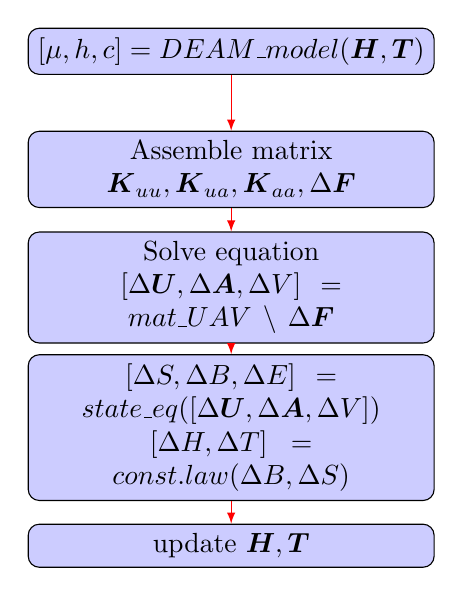
\begin{tikzpicture}[node distance = 1.5cm, auto]
            %\node[block]                  (t1){$\mathbf{H}=\boldsymbol{0}$, $\boldsymbol{T}=\boldsymbol{0}$, $n=1$};
            \node[block]   (t1){ $[\mu,h,c]=DEAM\_model(\boldsymbol{H},\boldsymbol{T})$};
           % \node[block, below of=t2](t3){update coefficient to finite element};
            \node[block, below of=t1]   (t2){Assemble matrix $\boldsymbol{K}_{uu},\boldsymbol{K}_{ua},\boldsymbol{K}_{aa}, \Delta\boldsymbol{F}$};
            %\node[block, right=0.5cm of t4, anchor=west]   (t6){compute $\Delta\mathbf{B}$, then extract $\Delta\mathbf{H},\Delta\mathbf{T}$, from $\Delta\mathbf{B},\Delta\mathbf{U}$ and update $\mathbf{H}=\mathbf{H}+\Delta\mathbf{H}$, $\mathbf{T}=\mathbf{T}+\Delta\mathbf{T}$};
            %\node[decision, above right=0.05cm and 2cm of t2, anchor=west](t7){Check $n=N$};
            %\node[block, above of=t7, text width=5em]   (t8){$n=n+1$};
            \node[block, below of=t2]   (t3){Solve equation \\ $[\Delta\boldsymbol{U},\Delta\boldsymbol{A},\Delta V]=mat\_UAV \setminus \Delta\boldsymbol{F}$};
            %\node[block, right=0.5cm of t5, anchor=west]   (t9){Chose $\Delta\mathbf{H}_{dc}$, $N=\mathbf{H}_{dc} \setminus \Delta\mathbf{H}_{dc}$ \\ assemble differential external load $\Delta\mathbf{F}$};
            %\node[block, right=2cm of t7, anchor=west] (t10){Solve FEM equation under $\mathbf{H}_{ac}$};
            \node[block, below=2cm of t3, anchor=south]   (t4){$[\Delta S, \Delta B, \Delta E] = state\_eq([\Delta\boldsymbol{U},\Delta\boldsymbol{A},\Delta V])$ \\ $[\Delta H, \Delta T] = const.law(\Delta B, \Delta S)$};
            \node[block, below of=t4]   (t5){update $\boldsymbol{H}, \boldsymbol{T}$};

            \path[line] (t1) --          (t2);
            \path[line] (t2) --          (t3);
            \path[line] (t3) -- 		 (t4);
            \path[line] (t4) -- 		 (t5);
            %\path[line] (t5) -- 		 (t6);
            %\path[line] (t6.north)   -|		 (t7);
            %\path[line] (t7) -- node{no} (t8);
            %\path[line] (t7) -- node{yes} (t10);
            %\path[line] (t8) |-		 ($(t2.north) + (0,3mm)$);
            %\path[line] (t9) -- 		 (t5);

        \end{tikzpicture}%
   \end{column} 
\end{columns}	
\end{frame}


\subsection{Dynamic analysis}
\begin{frame}\frametitle{Dynamic analysis}
%\vspace{-10.5pt}
\begin{itemize}[label=$\bullet$, font=\small, leftmargin=*]
\item \textbf{Elastic equilibrium}
\begin{equation*}
	\text{div }\boldsymbol{T} + \boldsymbol{f} = \rho \frac{d^2 \boldsymbol{u}}{dt^2}
	\hspace{2cm} \rho \text{: masse volumique kg/m}^3
	\end{equation*}

\item \textbf{Ampere's law}
\begin{equation*}
				\left\{ 
				\begin{aligned}
				\text{curl } \boldsymbol{H} & = \boldsymbol{J}_c \\
				\text{div } \boldsymbol{J}_c & = 0
        		\end{aligned}
				\right.
				\hspace{2cm} \boldsymbol{J}_c = \sigma_c \boldsymbol{E} \text{: eddy currents}
	\end{equation*}
Introduce time primitive of electric potential
\begin{equation*}
\boldsymbol{E} = - \frac{d(\boldsymbol{a}+ \text{grad }\psi)}{dt}
\hspace{2cm} \text{with } V=\frac{d \psi}{dt}
\end{equation*}
\item \textbf{Gauss's law}
\begin{equation*}
\frac{d(\text{div } \boldsymbol{D})}{dt} = 0
\hspace{0.5cm} \text{for the symetry of the system} 
\end{equation*}
\end{itemize}
\end{frame}

\begin{frame}\frametitle{Linear harmonic analysis}
%\vspace{-10.5pt}
\begin{beamercolorbox}[center]{equation}
      \begin{equation*}
		[\mathbb{K}] \{ X \}=[F]
		\end{equation*}
\end{beamercolorbox}
with:
\begin{itemize} [label=$\bullet$, font=\small, leftmargin=*]
{\small
\item  \begin{equation*} 
[\mathbb{K}] = \begin{bmatrix}
       {\color{brown}-\omega^2\boldsymbol{M}_{uu} + j\omega\boldsymbol{C}_{uu}} + \boldsymbol{K}_{uu} & - \boldsymbol{K}_{ua} & j\omega\boldsymbol{K}_{u\psi} & 0\\[0.3em]
       -\boldsymbol{K}_{ua}^t & {\color{blue}j\omega\boldsymbol{C}_{aa}} + \boldsymbol{K}_{aa} & {\color{blue}j\omega\boldsymbol{C}_{a\psi}} & 0 \\[0.3em]
       j\omega\boldsymbol{K}_{u\psi}^t & {\color{blue}j\omega\boldsymbol{C}_{a\psi}^t} & {\color{blue}j\omega\boldsymbol{C}_{\psi \psi}} + \omega^2\boldsymbol{K}_{\psi \psi} & {\color{magenta}-j\omega\boldsymbol{K}_{\psi q}} \\
       0 & 0 & {\color{magenta}-j\omega\boldsymbol{K}_{\psi q}^t} & {\color{magenta}j\omega Z}
\end{bmatrix}
\end{equation*}
}
\item $\{ X \} = \{\boldsymbol{u},\hspace{0.2cm} \boldsymbol{a},\hspace{0.2cm} \psi,\hspace{0.2cm} Z \}^t$.
\end{itemize}
\begin{columns}[totalwidth=\textwidth] 
	\begin{column}{.5\textwidth}  
$Z$ : Electrical charge connecting two electrodes.
	\end{column}
	\begin{column}{.4\textwidth}  
\includegraphics[width=0.95\textwidth]{Graphic/01_geoMEcircu.pdf}
	\end{column}
	\end{columns}
\end{frame}

\section{Laminate}
\subsection{Laminate composite with circular section}

\begin{frame}\frametitle{Geometry}
%\vspace{-10.5pt}
\begin{columns}[totalwidth=\textwidth] 
	\begin{column}{.68\textwidth}  
	\begin{exampleblock}{Why laminate composite?}
	 \begin{itemize} [label=$\boxed{\checkmark}$, font=\small, leftmargin=*]
	 \item Good coupling can be obtained at the ferroelectric and ferromagnetic interfaces.
	 \item Higher resonance response in a wide frequency range
	 \end{itemize}
	\end{exampleblock}
	\end{column}
	\begin{column}{.3\textwidth}  
\refonslide{Wang, Lei, et al.}{Effect of load resistance on magnetoelectric properties in FeGa/BaTiO3/FeGa laminate composites.}{Journal of Alloys and Compounds 509.30 (2011): 7870-7873.}
	\end{column}
	\end{columns}
\vspace{0.3cm}	
\begin{columns}[totalwidth=\textwidth]
   \begin{column}{.49\textwidth}
       \begin{beamercolorbox}[sep=8pt,center]{equation}
      Mode TT 
      \end{beamercolorbox}
\centering \includegraphics[height=3cm,width=0.9\textwidth]{Graphic/03_circuitTT.pdf}
   \end{column}
   \begin{column}{.49\textwidth}
       \begin{beamercolorbox}[sep=8pt,center]{equation}
      Mode LT 
      \end{beamercolorbox}
\centering \includegraphics[height=3cm,width=0.9\textwidth]{Graphic/03_circuitLT.pdf}
   \end{column}
\end{columns}
\centering
{\small
BaTiO$_3$ (gray layer): Thickness 1.5mm, diameter 12mm \\
FeGa (magenta layer): Thickness 1mm, diameter 10mm	
}
\end{frame}

\begin{frame}\frametitle{DC magnetic field dependence}
%\vspace{-5.5pt}
\Wider[4em]{
\begin{columns}[totalwidth=\textwidth]
   \begin{column}{.52\textwidth}
       \centering
       Simulation result
        \includegraphics[height=0.65\textwidth ,width=0.95\textwidth]{Graphic/result_nonlinear.pdf} \\
   \end{column}

   \begin{column}{.48\textwidth}
   \centering
   Measurement
   \includegraphics[height=0.65\textwidth ,width=0.95\textwidth]{Graphic/03_result_expe.pdf}
   \end{column}
   
\end{columns}
}
\begin{itemize}[label=$\bullet$, font=\small, leftmargin=*]
       \item ME voltage coefficient as a function of DC magnetic field under various electrical resistance load values and external magnetic field: $H_{ac}=1$ (Oe), $f=1$ (kHz)
		\item In concordance with \refonslide{Wang, Lei, et al. 2011.}{Effect of load resistance on magnetoelectric properties in FeGa/BaTiO3/FeGa laminate composites.}{Journal of Alloys and Compounds}
\end{itemize}
\end{frame}

\begin{frame}\frametitle{Eddy current effect}
%\vspace{-10.5pt}
\Wider[3em]{
\begin{columns}[totalwidth=\textwidth]
   \begin{column}{.49\textwidth}
   \centering
   TT mode
       \includegraphics[height=0.49\textwidth ,width=0.99\textwidth]{Graphic/TT_compare_eddy.pdf}
      \end{column}
   \begin{column}{.49\textwidth}
   \centering
   LT mode
       \includegraphics[height=0.49\textwidth ,width=0.99\textwidth]{Graphic/LT_compare_eddy.pdf}
     \end{column}
\end{columns}
}
\begin{columns}[totalwidth=\textwidth]
 \begin{column}{.59\textwidth}
\begin{itemize}[label=$\bullet$, font=\small, leftmargin=*]
\item The magnetic external field: $H_{ac}=1$ (Oe)
\item The result with effect of eddy current in TT mode in concordance with measurment 
\item The quality factor decrease under eddy current effect.
\end{itemize}
\end{column}
\begin{column}{.39\textwidth}
\centering
\includegraphics[width=0.79\textwidth]{Graphic/03_potencircle}
{\small Electrical potential distribution}
\end{column}
\end{columns}
\end{frame}

\begin{frame}\frametitle{Performance}
%\vspace{-10.5pt}
\begin{columns}[totalwidth=\textwidth]
   \begin{column}{.49\textwidth}
       \begin{block}{TT mode}
    {
        \includegraphics[height=0.4\textwidth ,width=0.99\textwidth]{Graphic/TT_compare_power.pdf}
    }
    \end{block}

   \end{column}
   \begin{column}{.49\textwidth}
       \begin{block}{LT mode}
    {
        \includegraphics[height=0.4\textwidth ,width=0.99\textwidth]{Graphic/LT_compare_power.pdf}
    }
    \end{block}
   \end{column}
\end{columns}
\begin{itemize}
\item Output power $P=V^2/R$ (post processing)
\item The eddy current decrease the performance of material.
\item Measurement with $P_{max}=2.75(\mu W)$ $R_{opt}=0.6 k\Omega$
\end{itemize}
\end{frame}

\begin{frame}\frametitle{Geometry}
%\vspace{-10.5pt}

\end{frame}











\section{Conclusion}
\begin{frame}\frametitle{Conclusion and perspectives}
\begin{block}{Conclusion}
\begin{itemize}
\item Completed FEM of circular tri-laminated ME composite has been presented.
\item The effect of eddy current is included.
\item The 3D analysis provides a useful tool to study ME composite of various geometries for energy transducer.
\end{itemize}
\end{block}
\begin{exampleblock}{Perspectives}
\begin{itemize}
\item Optimization geometry can be performed by this model.
\item Investigation under large signal of magnetic field 
\item Time reduction for computation is needed.
\end{itemize}
\end{exampleblock}
\vspace*{0.5cm}
\centering {\color{red}\textbf{\huge THANK YOU FOR YOUR ATTENTION}}
\end{frame}

%\section*{References}
%\begin{frame}[allowframebreaks]
%%\fontsize{9pt}{7.2}\selectfont
%        \bibliographystyle{plainnat}
%        \bibliography{biblio}
%\end{frame}
\end{document}
